\documentclass[class=report, crop=false, a4paper, 12pt]{standalone}

%Packages import
\usepackage{../pkgs}


\begin{document}
\par From the previously described systems in Section~\ref{sec:related_work}, two methods must be picked: one for face detection and one for face representation (that include the feature extracting backbone neural network and the loss function necessary for training). The next sections describe these choices and the reasons behind them, as well as the implementation and necessary steps.

\section{Face detection}
\par Following the proposed pipeline for a Face Recognition system, the initial design choice pertains to the Face Detection module, responsible for detecting, selecting and standardizing the faces. A comprehensive study of solutions was presented in \hyperref[sec:face_detect]{Section 2.3.1} and complemented with \hyperref[appendix:face_detection_appendix]{Appendix A}, wherein RetinaFace emerged as the most adequate solution for a student monitoring context, therefore, it will be the method used in this work. This approach accepts an image as input and produces multiple outputs, including a bounding box, five key facial landmarks (representing the center of the eyes, nose, and corners of the mouth), and a confidence score that reflects the likelihood of the detection accurately identifying a face. The selection of this method was predominantly influenced by three critical factors: 1) adaptability to changes in light, pose, facial expressions, etc., facilitated by the DCNN backbone, 2) incorporation of a single-stage approach and leveraging multi-task learning, enabling efficient real-time detection of facial landmarks using just a single CPU core (for VGA resolution), and 3) availability of readily implemented solutions with ample support.

\par The solution of choice is a Pytorch implementation\footnote{\url{https://github.com/biubug6/Pytorch_Retinaface}} of the original method that offers both a MobileNet-0.25 or ResNet-50 as backbones pre-trained on ImageNet. To better suit our application, further development over the original implementation was required. RetinaFace is distributed as a general face detection algorithm that is deployed on data with multiple faces to be handled, therefore, there is no built-in method for face selection or transformations, like alignment and resizing. However, on a student's monitoring scenario, only one face is relevant, and as consequence of that, the face recognition systems are to be trained and validated on single face pictures normalized to a canonical view.

\begin{figure}[!h]
    \centering
    \includegraphics[width=0.9\textwidth]{RF_1_crop.jpg}
    \caption[Results produced by the RetinaFace method over a test photo.]{Results produced by the RetinaFace method over a test photo. Represented are the bounding boxes, respective confidence scores and the five facial landmarks.}
    \label{fig:rf_1}
\end{figure}

Instantiating the model with default threshold parameters and Resnet-50 as the backbone, it produces the results seen in \reffig{fig:rf_1}. From all the bounding boxes available, one must be picked, and one way of doing so is by assuming that the more relevant face is closer to the camera, hence the area of its bounding box will be greater.

\begin{figure}[H]
    \centering
    \begin{minipage}[c]{0.48\textwidth}
      \centering
      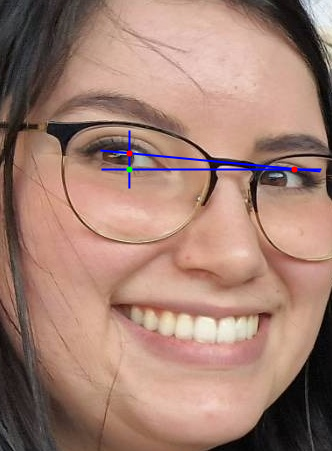
\includegraphics[width=0.7\textwidth]{RF_2.png}
      \label{fig:rf_2}
    \end{minipage}
    \hfill
    \begin{minipage}[c]{0.48\textwidth}
      \centering
      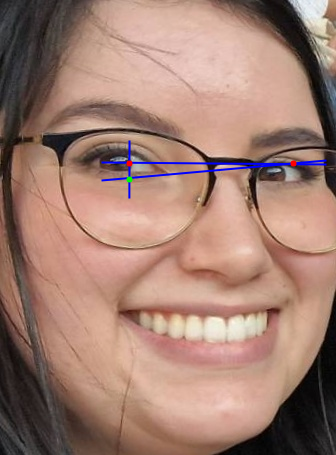
\includegraphics[width=0.7\textwidth]{RF_3.png}
      \label{fig:rf_3}
    \end{minipage} 
    %\vspace{-0.4cm}
    \caption[Visualization of the developed landmark-based alignment.]{Visualization of the developed landmark-based alignment. The green dot serves as an auxiliary point, resulting from the intersection of a horizontal line originating at the pivot eye and a vertical line projected from the other eye. Subsequently, the rotation angle is determined by computing the arctangent of two distances: the distance between the higher eye and the auxiliary point, and the distance from the auxiliary point to the pivot eye.}
    \label{fig:rf_2_3}
\end{figure}

\par The alignment is done with the help of the eyes landmarks as seen in \reffig{fig:rf_2_3}. The eye lower relative to the other is declared as the pivot and starting point of a horizontal line that acts as the reference to calculate the angle of rotation. Following the selection, cropping, and alignment of the face, it is resized to fit the required dimensions of the subsequent phase.

\section{Face Representation}
The Face Representation stage addresses handling the features of each face and includes a feature extractor and a loss function. Following the review on related works in \hyperref[appendix:related_work]{Section 2.5} Ganidisastra and Bandung~\autocite{ganidisastraIncrementalTrainingDeep2021} and SMOWL~\autocite{labayenOnlineStudentAuthentication2021} both utilize Facenet trained with triplet loss for face recognition. This naturally prompts an investigation into the potential effects on performance when utilizing a modern network (ResNet variations), as well as a lightweight network with fewer parameters (MobileFaceNet). Furthermore, considering the drawbacks associated with triplet loss training, examining the impact of a well-established loss function, like ArcFace would also be noteworthy, as it encourages intra-class compactness and inter-class distance. Due to time constraints, the methods of choice are all pretrained and subsequently fine-tuned on datasets appropriate to the model's scenario deployment.

\subsection{FaceNet}
For this method, we utilize a highly regarded PyTorch implementation\footnote{https://github.com/timesler/facenet-pytorch} that offers pretrained models in either the CASIA-WebFace or VGGFace2 dataset. The images' faces are cropped and aligned (but not rotated) using MTCNN, and resized to $160\times160\times3$. However, this implementation has differences compared to the Facenet described in the original paper~\autocite{schroffFaceNetUnifiedEmbedding2015}. Firstly, differing from the original adopted GoogLeNet-style Inception model, the backbone network employed here is the Inception-Resnet-V1, which integrates residual blocks into the Inception architecture. As highlighted in \hyperref[sec:resnet]{Section 2.4.2}, this modification streamlines the training process by addressing issues such as accuracy degradation and gradient vanishing. Secondly, adhering to the recommendations by Parkhi \textit{et al.}~\autocite{parkhiDeepFaceRecognition2015}, the network was trained as a classifier using softmax loss, departing from the original's triplet loss metric learning approach. Finally, the method's output is a 512-dimensional embedding, differing from the 128-dimensional output reported in the original paper.

\subsection{ResNet}
The choices for this architecture were designed to cover a range of neural network depth, complexity and trainable parameters. Henceforth, there are 3 objects of study, ranging from less to deeper ones: iResnet-18\footnote{\url{https://github.com/deepinsight/insightface}}, a 29 layer version of Resnet-34\footnote{\url{http://dlib.net/face_recognition.py.html}} (used in the TrustID project) and iResnet-50 (with \acrshort{SE} blocks)\footnote{\label{fnote6}\url{https://github.com/TreB1eN/InsightFace_Pytorch}}. Both the iResnet-18 and iResnet-50 were trained on $112\times112\times3$ faces from the MS1MV2 dataset, using ArcFace as the loss function, and output 512-dimensional feature embeddings. Regarding the Resnet-34, it was trained with triplet loss on a custom dataset comprised of 3 million $150\times150\times3$ images from the Visual Geometry Group
Face~\autocite{parkhiDeepFaceRecognition2015} and FaceScrub~\autocite{ngDatadrivenApproachCleaning2014}, and outputs a 128-dimensional feature embedding.

\subsection{MobileFaceNet}
MobileFaceNet\cref{fnote6} is a lightweight approach to face recognition that will further aid the study of the computational cost and model's performance trade-off. Since it is made available by the same author as the iResnet-50, it has technical similarities. Once again, it is trained with ArcFace loss on $112\times112\times3$ images from the MS1MV2 dataset and outputs the usual 512-dimensional embedding.


\section{Finetuning data}
Considering that the intended application of the face recognition systems is to monitor students, the nature of the capture device (webcam or smartphone) or its positioning will influence the quality of the data. For instance, one potential scenario involves a student with one monitor and a laptop placed to the side of it, accompanied by a lamp on the opposite side. This will configuration will result in face captures with very different resolutions, poses and lightning compared to another student using a laptop, in a well lit room, facing the subject. 

\begin{figure}[H]
  \centering
  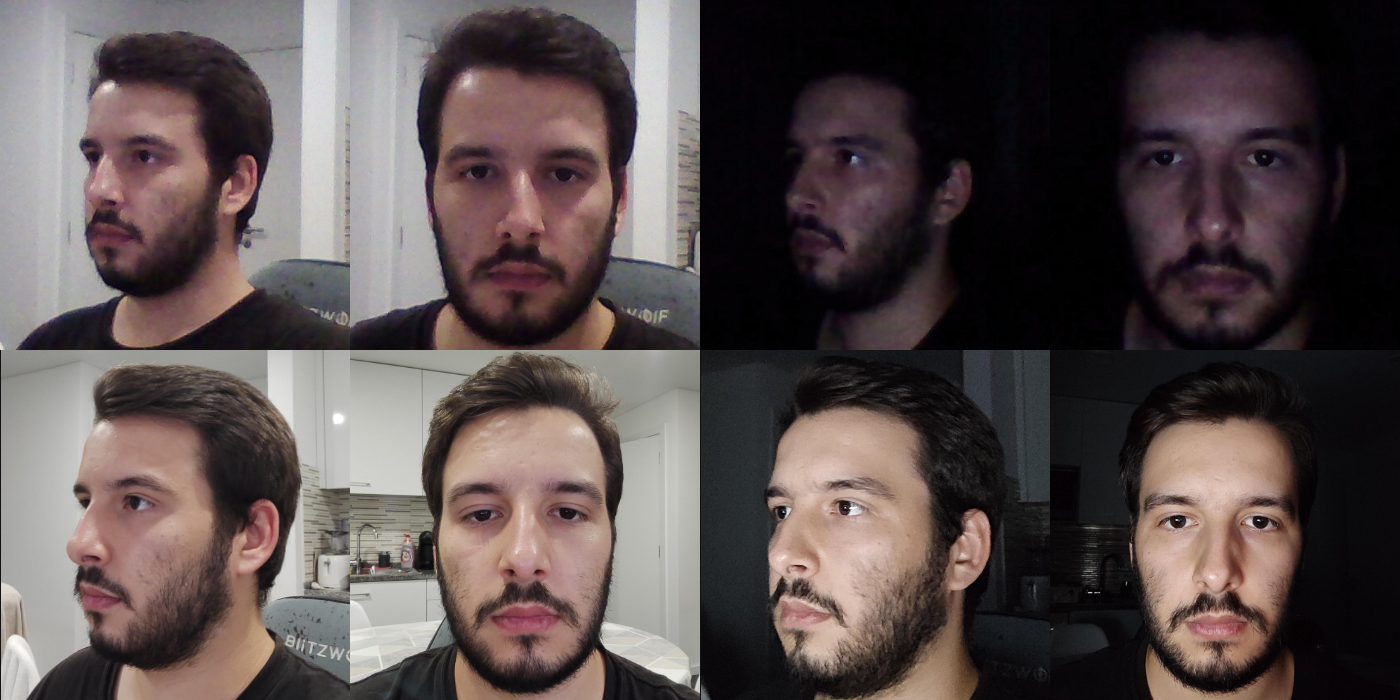
\includegraphics[scale=0.26]{scenarios.png}
  \caption[Comparison between devices for different face capturing scenarios.]{Comparison between devices for different face capturing scenarios. The top row corresponds to $1280\times720$ files captured by a webcam, while the bottom row are $2309\times3072$ pictures from a smartphone's front facing camera.}
  \label{fig:scenarios}
\end{figure}

As can be seen in \reffig{fig:scenarios}, for faces captured in the same exact scenarios and conditions there is a huge discrepancy between the webcam and smartphone pictures, ranging from resolution, detail, color and hue, and illumination. Therefore, it is crucial to have a robust system that is capable of being insensitive to these variations, hence the possible need to finetune pre-trained models for that. In this regard, we will examine two distinct datasets: DigiFace-1M and QMUL-SurvFace.

\begin{figure}[H]
  \centering
  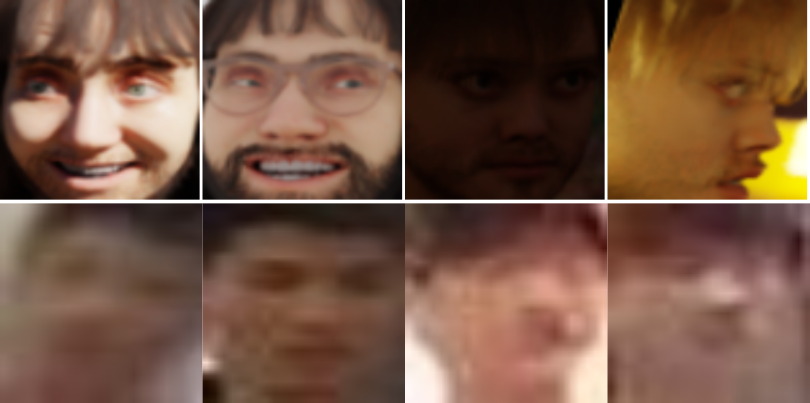
\includegraphics[scale=0.45]{ft_data.png}
  \caption[Examples of faces from the fine-tuning datasets.]{Examples of faces from the fine-tuning datasets. Row 1: QMUL-Survface, showcasing the low quality of the pictures. Row 2: DigiFace-1M, showcasing the variability in pose, color, accessories, expressions.}
  \label{fig:ft_data}
\end{figure}

\par Amidst the controversies surrounding the methods of data acquisition for some publicly distributed datasets, including MS-Celeb-1M, MegaFace, FaceScrub, IJB-C or VGGFace, Bae \textit{et al.} developed DigiFace-1M~\autocite{baeDigiFace1MMillionDigital2023} with those concerns in mind. This fully synthetic dataset emulates different scenarios with variant poses, light, expression and accessories (hats, masks, makeup, etc.), and it serves as an interesting object of study of the potential of this type of datasets to diminish the reliance over real face data to finetune a model for more adverse scenarios.
\par The second dataset used to finetune our models of choice is QMUL-SurvFace~\autocite{chengSurveillanceFaceRecognition2018} by Cheng \textit{et al}. Initially described as a benchmarking dataset, its unconstrained way of capturing resulted on faces with very high variance in resolution, capturing angles, poses, light or accessories, poses as a perfect source to further adapt the models to said scenarios. Another noteworthy benefit of this dataset is that the images were collected with the consent of the individuals, meaning that ethical and privacy dilemmas are not at play.

\section{Benchmarks}
\par The evaluation will be conducted with 10-fold cross validation on the processed dataset to match the size of the training data for each model. First with the original pretrained model and then with the fine-tuned version of the selected one. The model will produce the feature embeddings and pairwise cosine similarity, and if it is above a certain threshold the pair is considered as a match. 

\par To comprehensively assess the performance of the chosen models, we will subject them to testing across eight diverse datasets: VGGFace2, AgeDB30, two CFP variations (CFP-FF for frontal-frontal pairs and CFP-FP for frontal-profile pairs), CALFW, CPLFW, XQLFW and LFW. This approach is designed to capture a wide array of characteristics, closely resembling real-world scenarios for a thorough evaluation, therefore, four dataset groups based on their characteristics are defined: frontal, age, pose and hard. 


% \begin{table}[H]
%   \centering
%   \caption[Benchmarks' groups, their difficulty and intended evaluation purpose.]{Benchmarks' groups, their difficulty and intended evaluation purpose. * - Very easy. ***** - Very difficult.}
%   \label{tab:bench_groups}
%   \resizebox{0.5\textwidth}{!}{%
%   \begin{tabular}{c|c|c|c|}
%   \cline{2-4}
%   \multicolumn{1}{l|}{}                          & Dataset  & Difficulty & Evaluation purpose                                                                           \\ \hline
%   \multicolumn{1}{|c|}{\multirow{2}{*}{Frontal}} & CFP-FF   & ***        & \multirow{2}{*}{\begin{tabular}[c]{@{}c@{}}Frontal view\\ performance.\end{tabular}}        \\ \cline{2-3}
%   \multicolumn{1}{|c|}{}                         & LFW      & *          &                                                                                              \\ \hline
%   \multicolumn{1}{|c|}{\multirow{2}{*}{Age}}     & AgeDB30  & ***        & \multirow{2}{*}{\begin{tabular}[c]{@{}c@{}}Sensitivity to \\ age variations.\end{tabular}}   \\ \cline{2-3}
%   \multicolumn{1}{|c|}{}                         & CALFW    & ***        &                                                                                              \\ \hline
%   \multicolumn{1}{|c|}{\multirow{2}{*}{Pose}}    & CFP-FP   & ****       & \multirow{2}{*}{\begin{tabular}[c]{@{}c@{}}Performance for\\ a range of poses.\end{tabular}} \\ \cline{2-3}
%   \multicolumn{1}{|c|}{}                         & CPLFW    & ***        &                                                                                              \\ \hline
%   \multicolumn{1}{|c|}{\multirow{2}{*}{Hard}}    & VGGFace2 & *****      & \begin{tabular}[c]{@{}c@{}}Great variation in pose, \\ age, illumination, etc.\end{tabular}  \\ \cline{2-4} 
%   \multicolumn{1}{|c|}{}                         & XQLFW    & *****      & \begin{tabular}[c]{@{}c@{}}Performance for very\\ low image quality.\end{tabular}            \\ \hline
%   \end{tabular}%
%   }
%   \end{table}


% \begin{figure}[H]
%   \centering
%   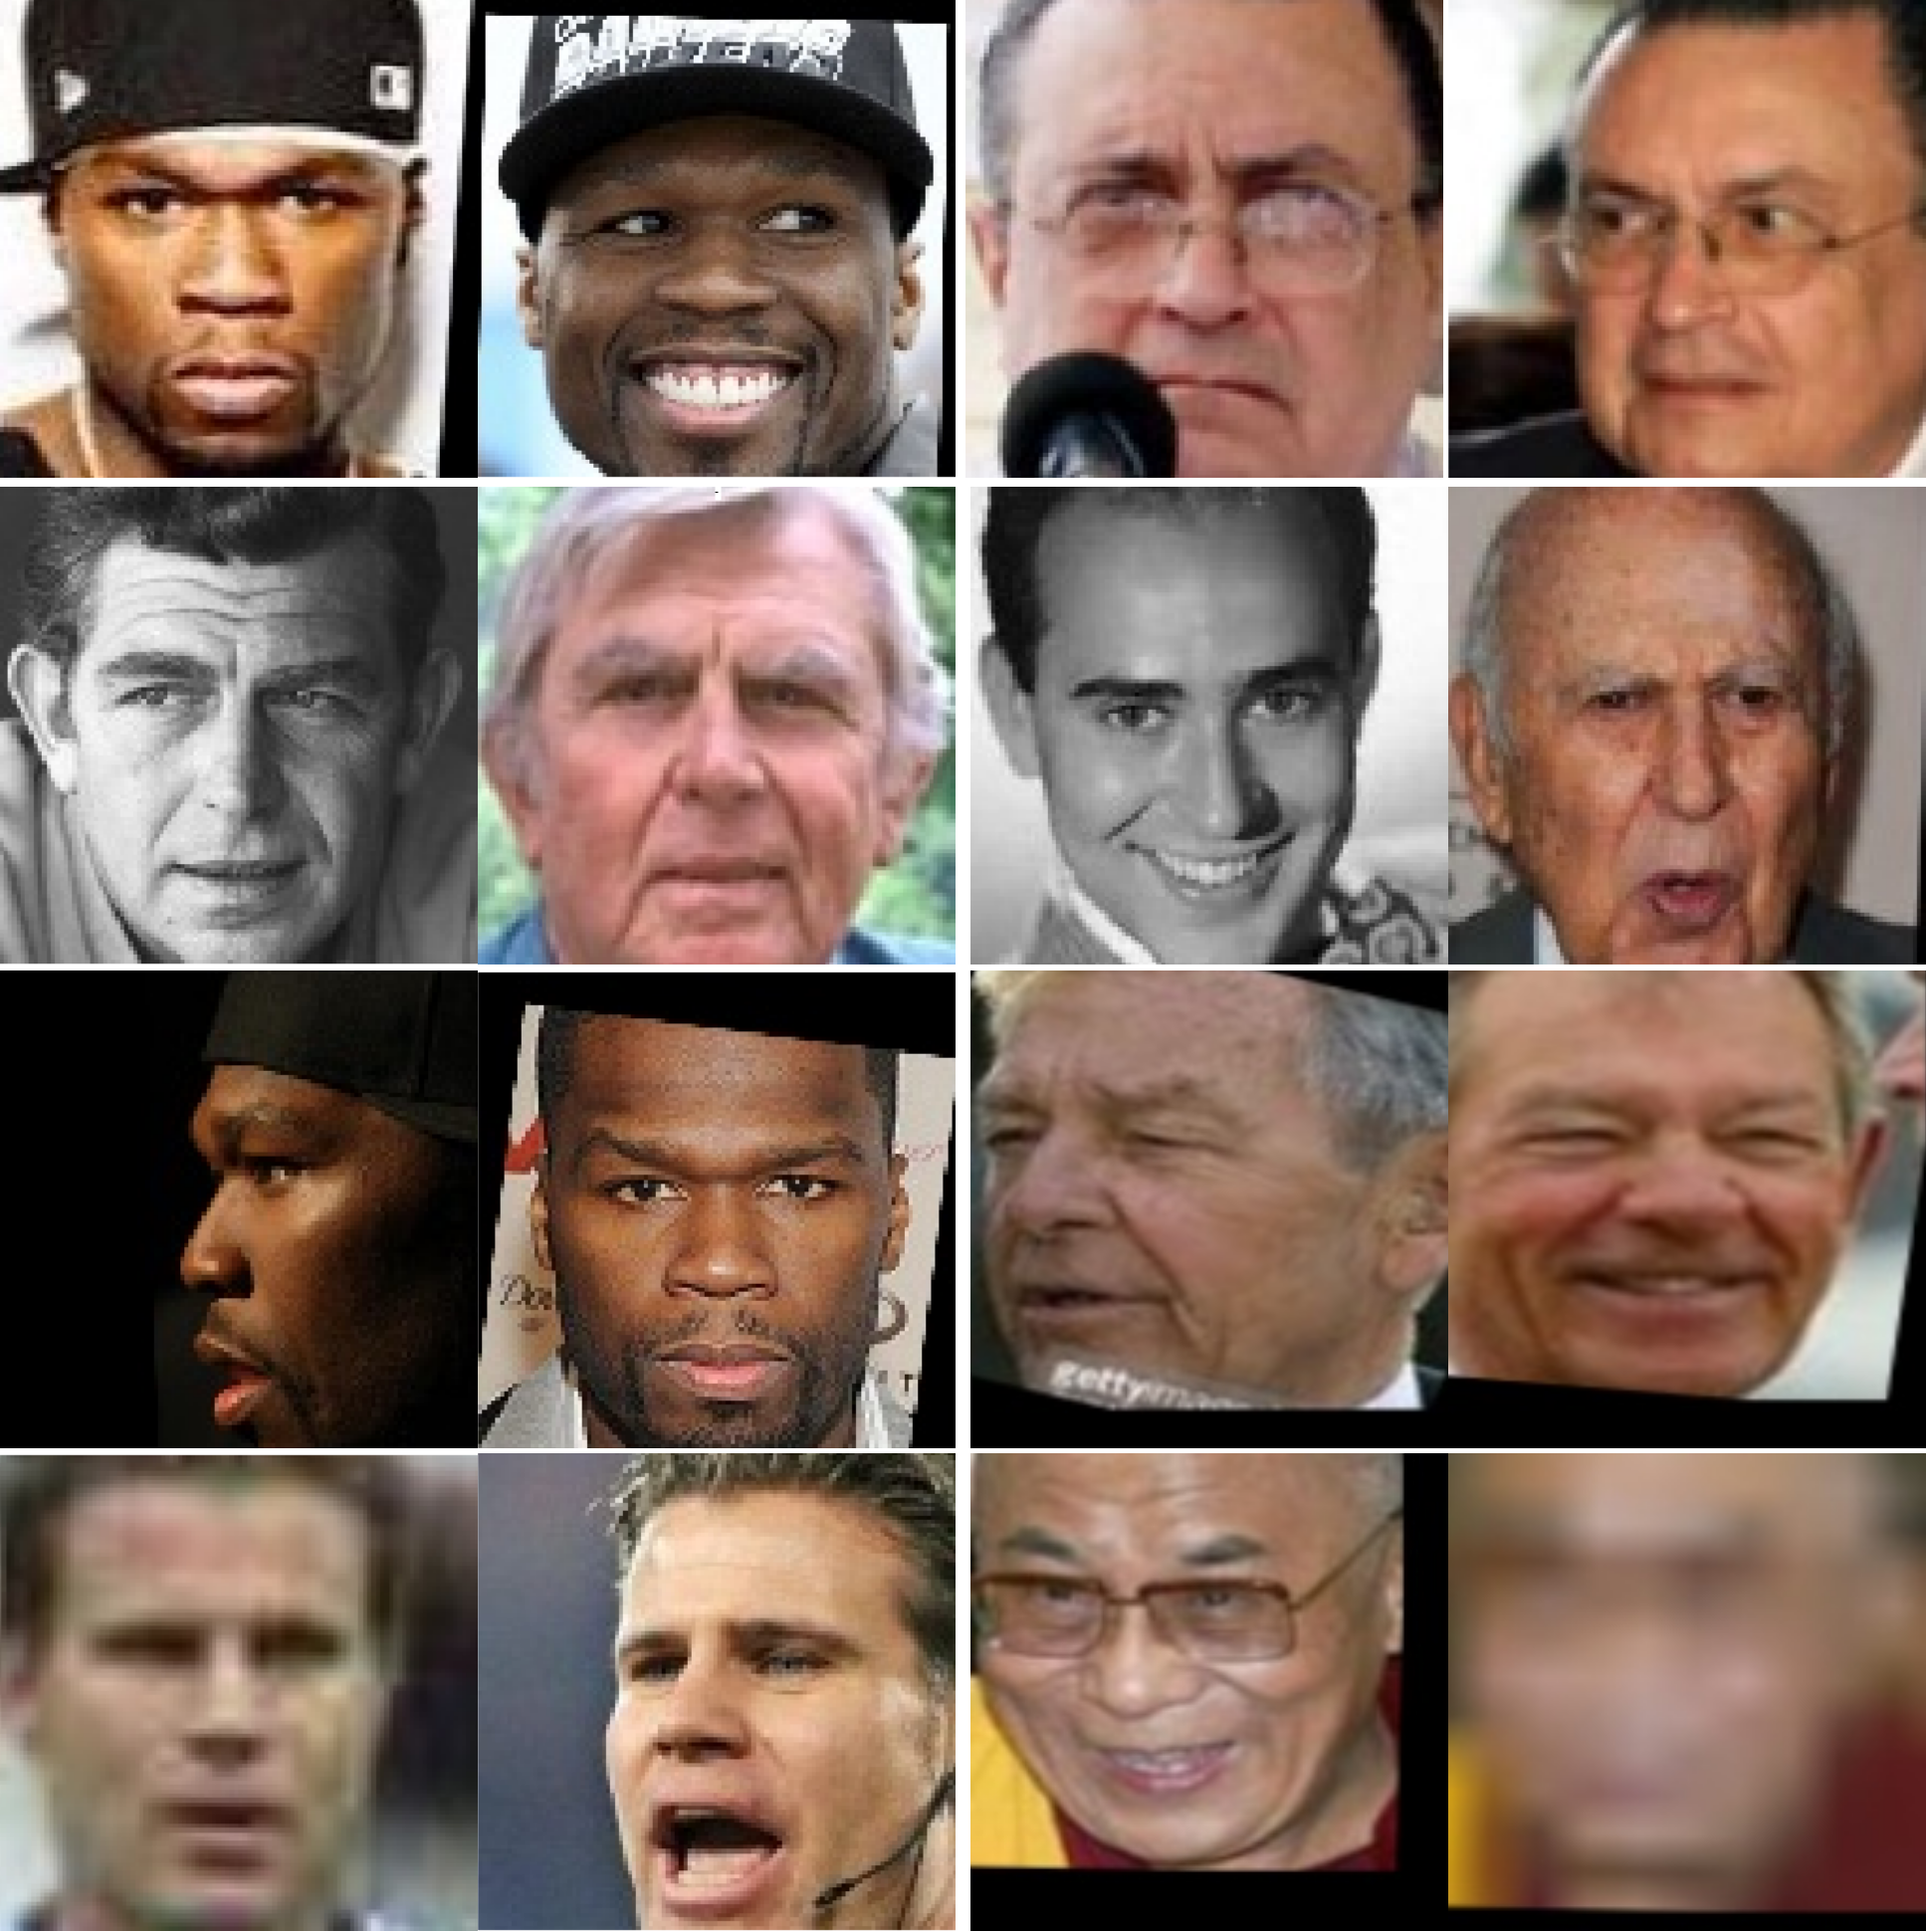
\includegraphics[scale=0.11]{benchmarks.png}
%   \caption[Example face pairs from each benchmark.]{Example face pairs from each benchmark. Row 1: CFP-FF and LFW; Row 2: AgeDB30 and CALFW; Row 3: CFP-FP and CPLFW; Row 4: VGGFace2 and XQLFW}
%   \label{fig:benchmarks}
% \end{figure}

\begin{figure}[H]
  \begin{minipage}{0.5\textwidth}
    \centering
    \begin{table}[H]
      \centering
      \caption[Benchmarks' groups, their difficulty, and intended evaluation purpose.]{Benchmarks' groups, their difficulty, and intended evaluation purpose. * - Very easy. ***** - Very difficult.}
      \label{tab:bench_groups}
      \resizebox{0.9\textwidth}{!}{%
        \begin{tabular}{c|c|c|c|}
          \cline{2-4}
          \multicolumn{1}{l|}{}                          & Dataset  & Difficulty & Evaluation purpose                                                                           \\ \hline
          \multicolumn{1}{|c|}{\multirow{2}{*}{Frontal}} & CFP-FF   & ***        & \multirow{2}{*}{\begin{tabular}[c]{@{}c@{}}Frontal view\\ performance.\end{tabular}}        \\ \cline{2-3}
          \multicolumn{1}{|c|}{}                         & LFW      & *          &                                                                                              \\ \hline
          \multicolumn{1}{|c|}{\multirow{2}{*}{Age}}     & AgeDB30  & ***        & \multirow{2}{*}{\begin{tabular}[c]{@{}c@{}}Sensitivity to \\ age variations.\end{tabular}}   \\ \cline{2-3}
          \multicolumn{1}{|c|}{}                         & CALFW    & ***        &                                                                                              \\ \hline
          \multicolumn{1}{|c|}{\multirow{2}{*}{Pose}}    & CFP-FP   & ****       & \multirow{2}{*}{\begin{tabular}[c]{@{}c@{}}Performance for\\ a range of poses.\end{tabular}} \\ \cline{2-3}
          \multicolumn{1}{|c|}{}                         & CPLFW    & ***        &                                                                                              \\ \hline
          \multicolumn{1}{|c|}{\multirow{2}{*}{Hard}}    & VGGFace2 & *****      & \begin{tabular}[c]{@{}c@{}}Great variation in pose, \\ age, illumination, etc.\end{tabular}  \\ \cline{2-4} 
          \multicolumn{1}{|c|}{}                         & XQLFW    & *****      & \begin{tabular}[c]{@{}c@{}}Performance for very\\ low image quality.\end{tabular}            \\ \hline
        \end{tabular}%
      }
    \end{table}
  \end{minipage}%
  \begin{minipage}{0.5\textwidth}
    \centering
    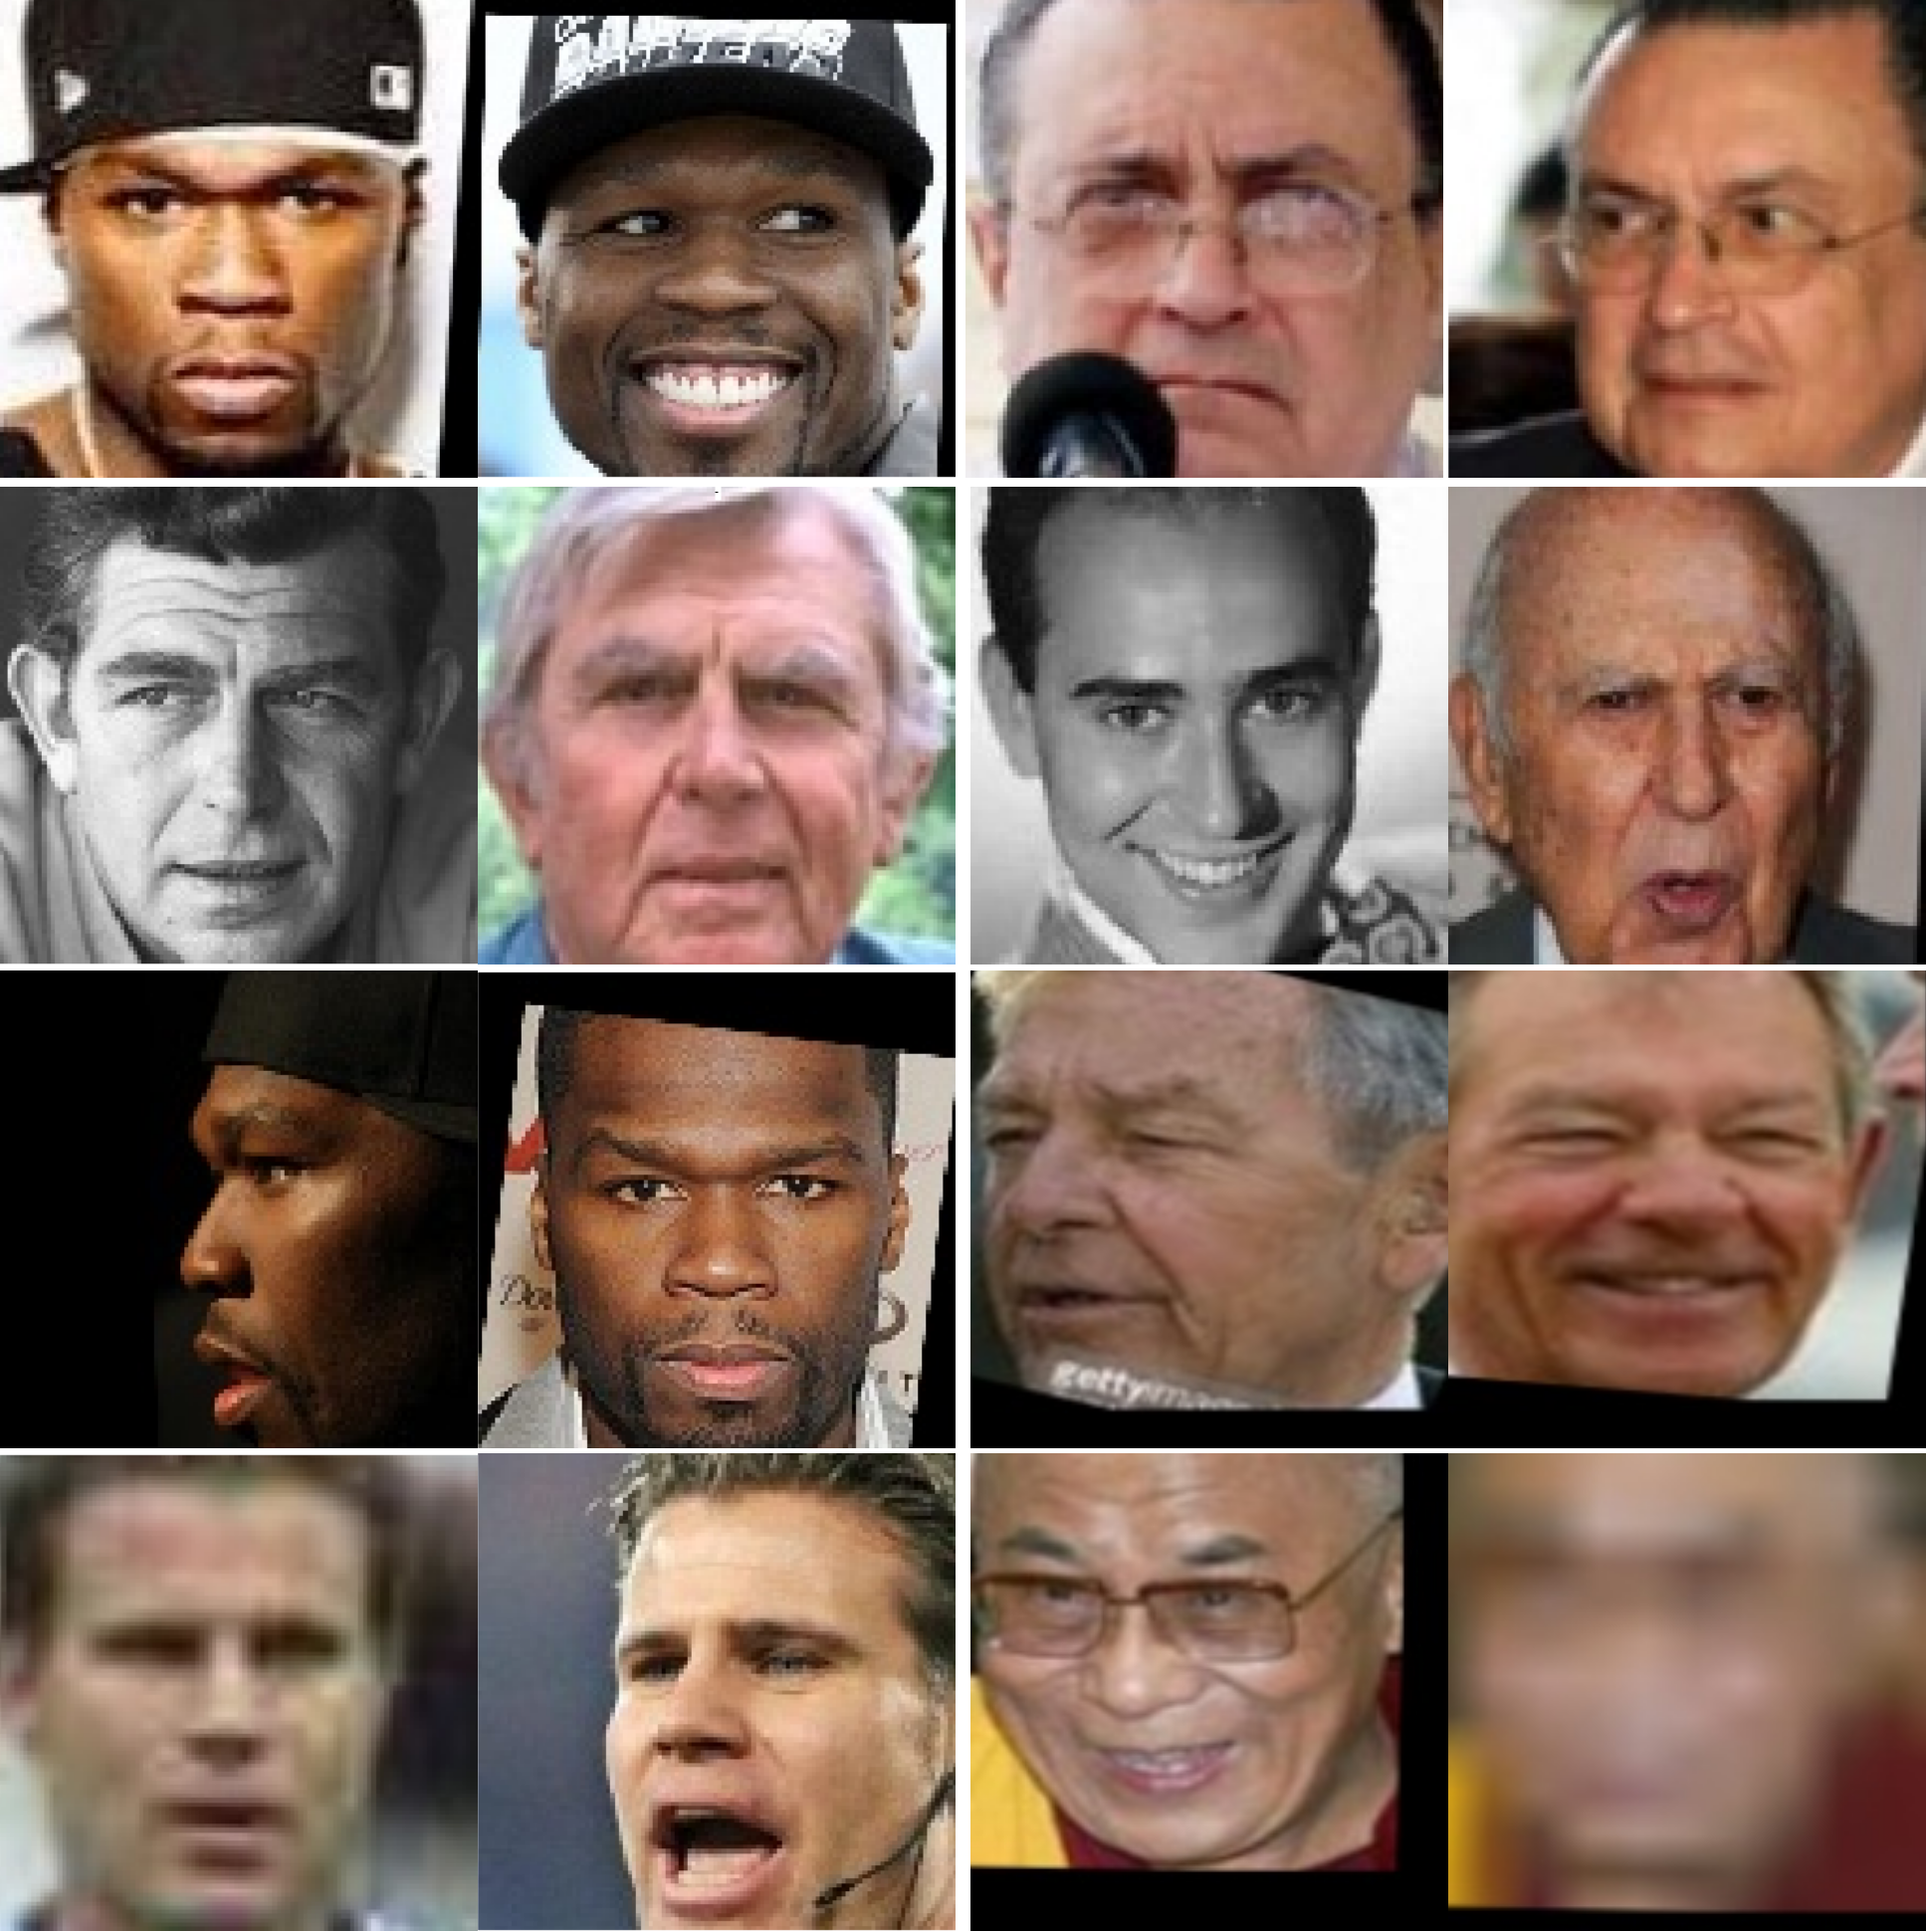
\includegraphics[width=0.95\textwidth]{benchmarks.png}
    \caption[Example face pairs from each benchmark.]{Example face pairs from each benchmark. Row 1: CFP-FF and LFW; Row 2: AgeDB30 and CALFW; Row 3: CFP-FP and CPLFW; Row 4: VGGFace2 and XQLFW}
    \label{fig:benchmarks}
  \end{minipage}
\end{figure}

  
These groups are summarized in \autoref{tab:bench_groups} and pictured on \reffig{fig:benchmarks}, where it is possible to observe the diversity in pose, expressions, age, illumination and image quality. In terms of difficulty, the Frontal group is easier, while the Age and Pose groups are moderate. However, the Hard group significantly raises the challenge, leading to stricter benchmarks.

% The frontal group is composed of the CFP-FF and LFW, easier datasets with only frontal views of the face. The age group is designed to evaluate the model's sensitivity to age variations, and gathers the AgeDB30 and CALFW datasets. The pose one measures the system's performance when tested against faces with a wide range of poses by evaluating in the CFP-FP and CPLFW datasets. Finally, the hard group includes VGGFace2, a large scale benchmark with great variation in pose, age, light, etc., and XQLFW, a very difficult dataset with degraded image quality. 

\par The chosen evaluation metrics are based on biometric systems of verification and encompass Accuracy, the \gls{ROC} and \gls{DET} plots obtained by sweeping an interval of thresholds and calculating the \gls{TAR}, \gls{FAR} and the \gls{FRR}, and the \gls{EER}.

\par Where TP is True Positive, TN is True Negative, FP is False Positive and FN is False Negative, the accuracy, a measure for the number of correct predictions, is computed by: 
\begin{equation}
  Accuracy=\frac{TP+TN}{TP+TN+FP+FN}
\end{equation}
Moreover, TAR and FAR, that indicate, respectively, the proportion of genuine face pairs correctly classified and the quantity of imposter face pairs incorrectly classified as matches, is determined by: 
\begin{equation}
  TAR=\frac{TP}{TP+FN}
\end{equation}
\begin{equation}
  FAR=\frac{FP}{FP+TN}
\end{equation}


\par With the previous metrics, it is possible to obtain the FRR, the ratio of genuine matches that are classified as a non-match:
\begin{equation} 
  FRR = 1 - TAR
\end{equation}  
Additionally, they also gives us the ability to plot the ROC curves and study the trade-off between the TAR and FAR at different thresholds and evaluate the performance of different models \reffig{fig:roc_curve}. With FRR, the DET curve are generated, which serves a similar purpose to the ROC curves, but with a better performance visualization due to the axis' logarithmic scale. Finally, the EER is the point where FRR = FAR and the lower it is, the better performing the system is. 


%\footnote{Commonly, FRR@FAR is also termed FNMR@FMR, yet they differ in "attempts" and "transactions" within a biometric system, where a transaction may comprise several attempts. Here, $FRR=FNMR$ and $FAR=FMR$ due to the absence of transactions or attempts.}

\begin{figure}[H]
  \centering
  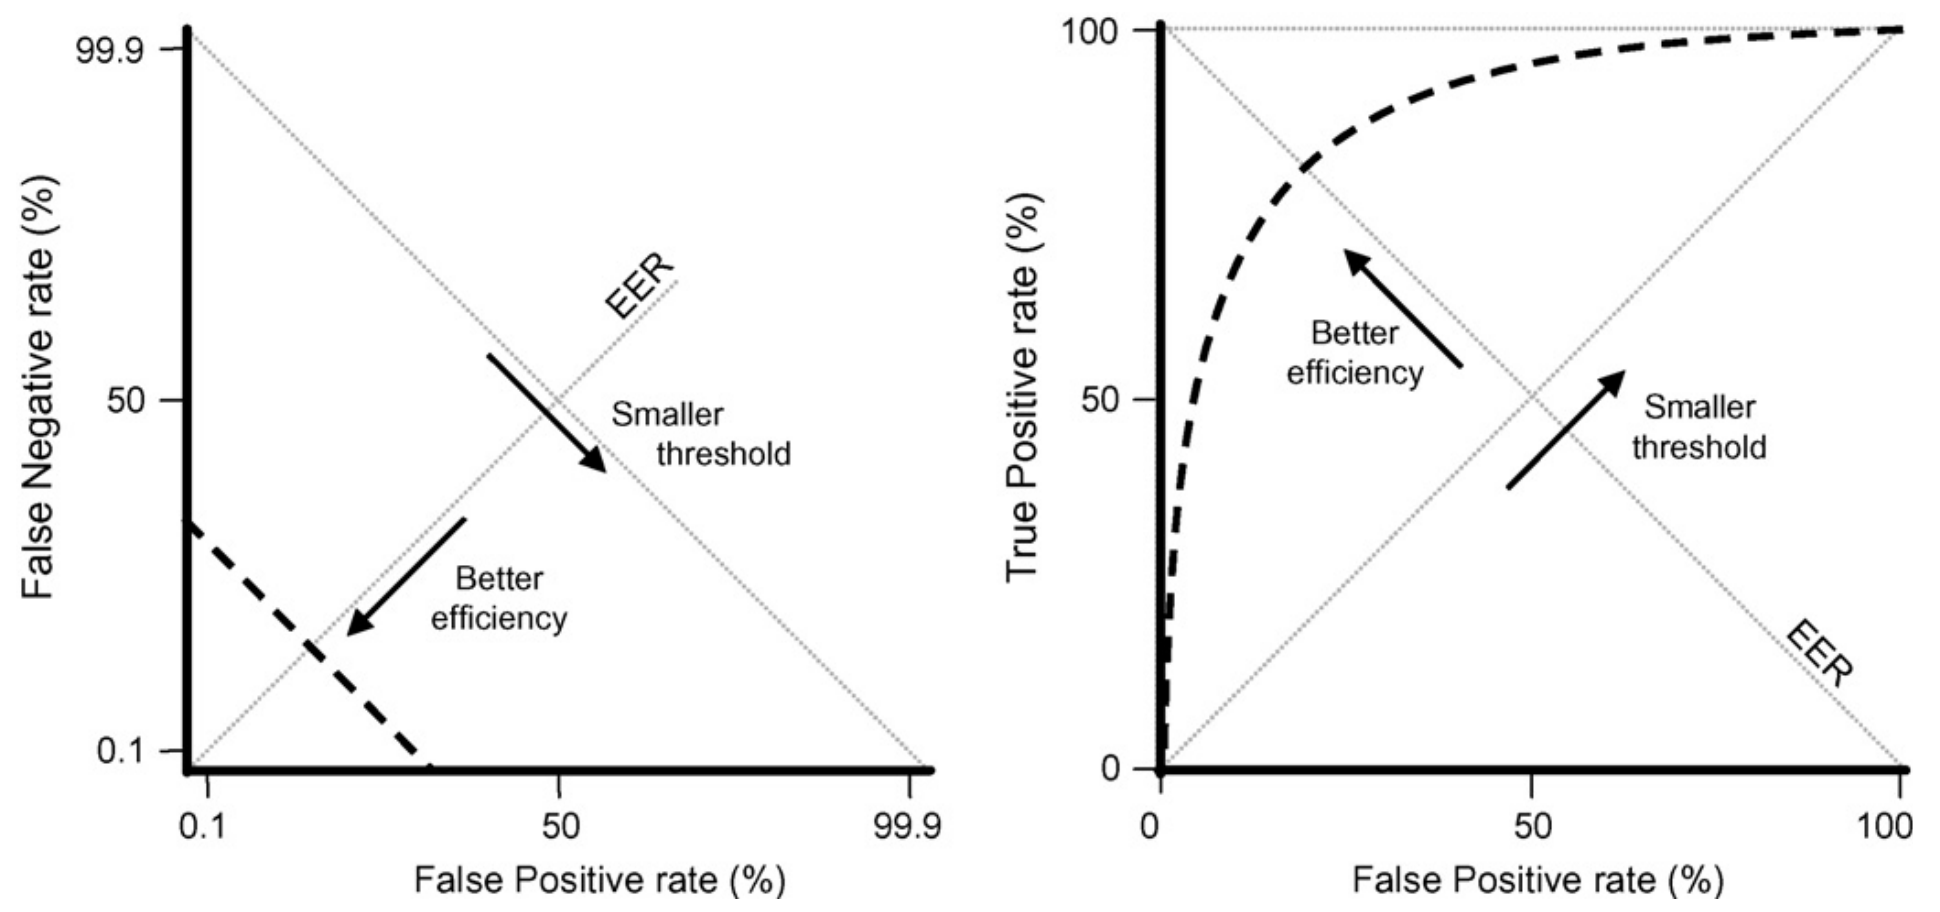
\includegraphics[scale=0.21]{roc_det.png}
  \caption[Range of possible performance for DET and ROC curves .]{Range of possible performance for DET (left) and ROC (right) curves. The y-axis represents the True Positive Rate (or TAR) for the ROC curves and False Negative Rate (or FRR) for the DET curves. The x-axis represents the False Positive Rate (or FAR) for both plots. Image from~\autocite{saenz-lechonMethodologicalIssuesDevelopment2006}}
  \label{fig:roc_curve}
\end{figure}

\par \reffig{fig:roc_curve} highlights the performance visualization for both the curves' plots. The closer the ROC curve is to the top left corner, the better performance the model has, since that means that it is able of correctly identify more genuine face matches (TAR) while minimizing the wrong identities incorrectly classified as matches (FAR). For DET, a curve closer to the origin represents a better model, since it minimizes the amount of genuine identities matches classified wrongly classified as imposters (FRR) for a more strict FAR threshold.
\par Furthermore, to evaluate the performance/resource utilization trade-off, the following are considered: the number of trainable parameters, trainable layers, quantity of multiplication and addition operations (mult-adds), inference time and a proposed metric called Number of Parameters per Unit of Accuracy (NPUA). 

\section{Implementation details}
\par All the training, processing, and benchmarking was developed in a Docker environment to ensure reproducibility. The code was written using Python 3.8.10 and relies on PyTorch 1.14.0 and Torchvision 0.15.0, along with their corresponding required libraries. The training process is conducted exclusively on a single GPU, specifically NVIDIA's GeForce RTX 3080 Ti 12GB. 
\par Regarding the implementation, all development was done with modularity in mind. First, the data is processed with the customized RetinaFace detection and alignment algorithm and saved. Then, it is proceeded forward to the neural network that produces a feature embedding for each image. If the model is being trained, the embedding will be passed on to the ArcFace module, which will output the feature's logits. Following the the original paper~\autocite{dengArcFaceAdditiveAngular}, the logits are turned to probabilities by applying the softmax activation function and then contributing to the final step, i.e, the cross entropy loss. Because ArcFace is a separate structure that does not integrate the backbone networks as a custom layer, the neural networks can be quickly and easily changed.

\section{Discussion}\label{sec:methodology_discussion}
\par Considering the possible challenging scenarios described allied to the incapability of guaranteeing robust computational power or quality capture devices, due to the image-based student monitoring application, it prompts a selection of the methods of face detection, recognition methods and training datasets with that in mind. 
\par RetinaFace's backbone DCNN assures adaptability to image variations resulting from the capture device, and its multi-task, real-time and single CPU core data processing eliminates the need for powerful execution machines. After being processed by the customized RetinaFace implementation, the datasets (QMUL-SurvFace and DigiFace-1M) will serve as a fine-tuning source. Their increased depth, width and varied image characteristics (accessories, illumination, poses, quality, etc.) constitute a theoretical robust source of diverse information to improve a model's competence. Finally, \hyperref[sec:related_work]{Section 2.5} highlighted FaceNet, iResnet-18, iResnet-SE-50 and MobileFaceNet as possible alternatives to TrustID's face recognition method. Since they are all deep learning approaches, they all have an inherent flexibility to adapt to information, but the data where they were trained has great influence on their performance. Regarding the computational power, these methods also differ in the overhead they generate, wherein iResnet-SE-50 is the heaviest and MobileFaceNet is the lightest. Hence, because they are trained on different datasets and have different complexity, each one must be benchmarked in order to pick the model to be fine-tuned that shows a better performance/resource utilization trade-off. Furthermore, it is important to acknowledge that achieving perfect accuracy is not an absolute requirement. This is because the monitoring process involves face verifications occurring over an extended period, during which a larger quantity of verifications can compensate for lower accuracy values.
\end{document}



